\documentclass{article}

\usepackage[margin=1in]{geometry}
\usepackage[colorlinks,linkcolor=blue,filecolor=blue,citecolor=magenta,urlcolor=blue]{hyperref}
\usepackage{bm,amsmath,amsthm,amssymb,multicol,algorithmic,algorithm,enumitem,graphicx,subfigure}
\usepackage{xargs}
\usepackage{stmaryrd}
\usepackage{natbib}


\newcommand{\algo}{\textsc{Spars-AMS}}





\begin{document}



\title{Sparsified Distributed Adaptive Learning with Error Feedback}

% \author{\textbf{Belhal Karimi, Xiaoyun Li, Ping Li} \\\\
% Cognitive Computing Lab\\
% Baidu Research\\
%   10900 NE 8th St. Bellevue, WA 98004, USA
% }

\date{}
\maketitle

\begin{abstract}
To be completed...
\end{abstract}

\section{Introduction}\label{sec:introduction}



\section{Method}\label{sec:main}

Consider standard synchronous distributed optimization setting. AMSGrad is used as the prototype, and the local workers is only in charge of gradient computation.


\subsection{TopK AMSGrad with Error Feedback}

References:

\citep{karimireddy2019error}
\citep{shi2019convergence}
\citep{stich2018sparsified}
\url{https://arxiv.org/pdf/1901.09847.pdf}
\url{https://proceedings.neurips.cc/paper/2018/file/b440509a0106086a67bc2ea9df0a1dab-Paper.pdf}
\url{https://pdfs.semanticscholar.org/8728/dee89906022c1d4f5c1de1233c3f65ab92f2.pdf?_ga=2.152244026.2027005181.1606271153-15127215.1603945483}


The key difference (and interesting part) of our TopK AMSGrad comprared with the following arxiv paper ``Quantized Adam''\url{https://arxiv.org/pdf/2004.14180.pdf} is that, in our model only gradients are transmitted. In ``QAdam'', each local worker keeps a local copy of moment estimator $m$ and $v$, and compresses and transmits $m/v$ as a whole. Thus, that method is very much like the sparsified distributed SGD, except that $g$ is changed into $m/v$. In our model, the moment estimates $m$ and $v$ are computed only at the central server, with the compressed gradients instead of the full gradient. This would be the key (and difficulty) in convergence analysis.


\begin{algorithm}[H]
\caption{\algo\ for Federated Learning} \label{alg:sparsams}
\begin{algorithmic}[1]

\STATE \textbf{Input}: parameter $\beta_1$, $\beta_2$, learning rate $\eta_t$. 
\STATE Initialize: central server parameter $\theta_{0} \in \Theta \subseteq \mathbb R^d$; $e_{t,i}=0$ the error accumulator for each worker; sparsity parameter $k$; $N$ local workers; $m_0=0$, $v_0=0$, $\hat v_0=0$

\FOR{$t=1$ to $T$}

\STATE\textbf{parallel for worker $i$ do}:
\STATE\quad Receive model parameter $\theta_{t-1}$ from central server
\STATE\quad  Compute stochastic gradient $g_{t,i}$ at $\theta_t$
\STATE\quad  Compute $\tilde g_{t,i}=TopK(g_{t,i}+e_{t,i},k)$
\STATE\quad  Update $e_{t+1,i}=e_{t,i}+g_{t,i}-\tilde g_{t,i}$
\STATE\quad  Send $\tilde g_{t,i}$ back to central server
\STATE \textbf{end parallel}

\STATE \textbf{Central server do:}
\STATE $\bar g_{t}=\frac{1}{N}\sum_{i=1}^N \tilde g_{t,i}$
\STATE $m_t=\beta_1 m_{t-1}+(1-\beta_1)\bar g_t$
\STATE $v_t=\beta_2 v_{t-1}+(1-\beta_2)\bar g_v^2$
\STATE $\hat v_t=\max(v_t,\hat v_{t-1})$
\STATE Update model$\theta_t=\theta_{t-1}-\eta_t\frac{m_t}{\sqrt{\hat v_t}}$

\ENDFOR
\end{algorithmic}
\end{algorithm}


\subsection{Convergence Analysis}
Nonconvex smooth loss function. Bounded gradient variance.

\subsubsection{Single machine}
We first define multiple auxiliary sequences. For the first moment, define

\begin{align*}
    &\bar m_t=m_t+\mathcal E_t,\\
    &\mathcal E_t=\beta_1\mathcal E_{t-1}+(1-\beta_1)(e_{t+1}-e_t),
\end{align*}
such that 
\begin{align*} 
    \bar m_t&=\bar m_t+\mathcal E_t\\
    &=\beta_1(m_t+\mathcal E_t)+(1-\beta_1)(\bar g_t+e_{t+1}-e_1)\\
    &=\beta_1\bar m_{t-1}+(1-\beta_1)g_t.
\end{align*}
TBD...

\subsubsection{Multiple machine}



\section{Experiments}\label{sec:experiment}
Our proposed TopK-EF with AMSGrad matches that of full AMSGrad, in distributed learning. Number of local workers is 20. Error feedback fixes the convergence issue of using solely the TopK gradient. 

\begin{figure}[h]
    \begin{center}
    \mbox{\hspace{-0.3in}
        \includegraphics[width=2.5in]{figure/mnist_cnn_test_accuracy.eps}
        \includegraphics[width=2.5in]{figure/cifar_cnn_test_accuracy.eps}
        \includegraphics[width=2.5in]{figure/cifar_lenet_test_accuracy.eps}
    }
    \end{center}
    \vspace{-0.1in}
	\caption{Test accuracy.}
	\label{fig:test accuracy}
\end{figure}



\section{Conclusion}\label{sec:conclusion}

\newpage

\bibliographystyle{plain}
\bibliography{ref}

\newpage
\appendix 

\section{Appendix}\label{sec:appendix}


%-----------------------------------------------------------------------------
%\vspace{0.4cm}

\end{document} 